%!TEX root = ../thesis.tex

\chapter{Conclusion}
\label{chp:conclusion}

Find an overview of this thesis as a whole in figure \ref{fig:overview}.
As a first step, the MINRV8 architecture inspired by the RISC-V architecture was defined and implemented in nuXmv in section \ref{sec:minrv8}.
In chapter \ref{chp:ifc}, information flow semantics and three information flow properties forming an information flow control in spirit of the work of \citeauthor{Ferraiuolo17} \cite{Ferraiuolo17} were developed.
The information flow semantics were used to augmented the model of the MINRV8 by information flow tracking.
In chapter \ref{chp:results} eight assumptions that, when implemented software running in machine-mode such as \glspl{os}, guarantee the absence of vulnerabilities covered by aforementioned information flow properties were presented.
Our model, the properties and the assumptions were evaluated by showing that taken together, they manage to detect both the cache poisoning \cite{Wojtczuk09} and the SYSRET vulnerability \cite{Dunlap19}.
Finally in chapter \ref{chp:discussion}, the limitations and the scope of our work were discussed and it was reflected whether our methodology is trustworthy.

\begin{figure}
    \centering
    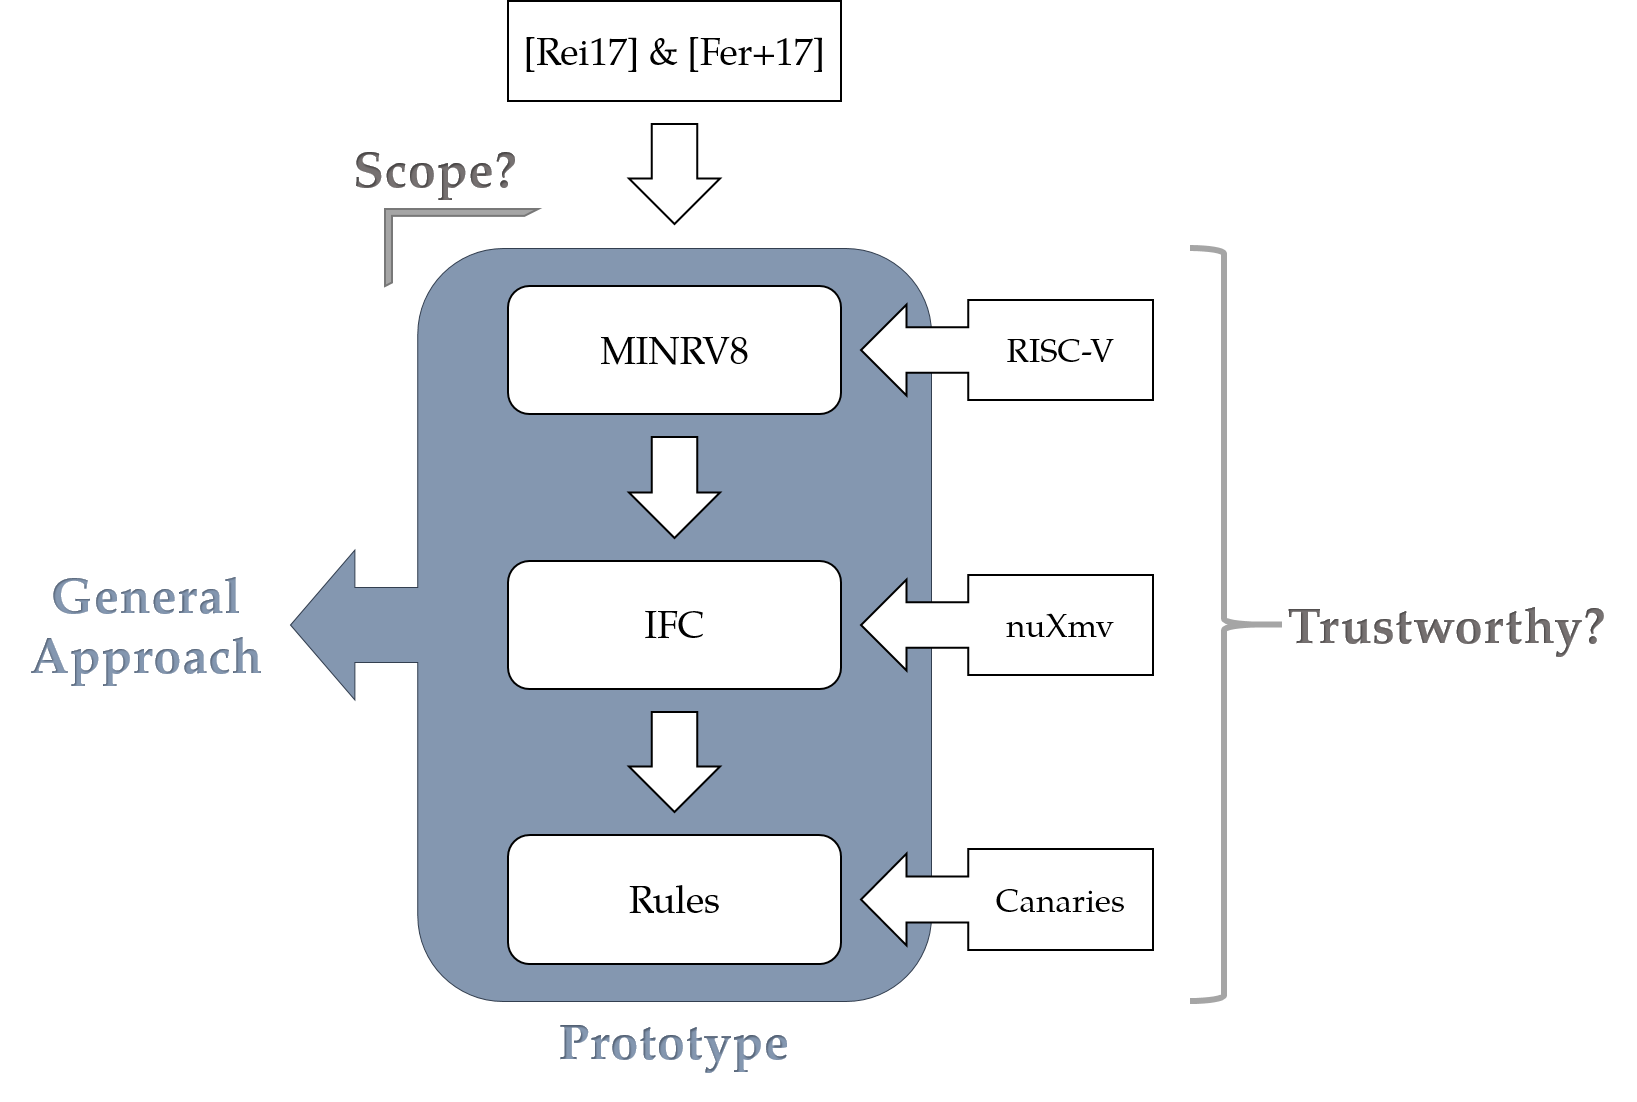
\includegraphics[width=\textwidth]{figures/thesis-overview.png}
    \caption{Thesis Overview}
    \label{fig:overview}
\end{figure}

Before a final summary of what has been achieved in this thesis will be given, we first recap all directions future work might take that were hinted towards throughout this thesis:
\begin{description}
    \item[Executable memory] First and foremost, the model could be enhanced by a model of executable memory to more closely resemble modern architectures.
    This was discussed extensively in section \ref{sec:discuss-arch}.
    \item[MMU] In light of \cite{KhakpourSD13} a model of an \gls{mmu} could be implemented to make use of information flow tracking on user-mode level.
    This was discussed in chapter \ref{chp:related-work}.
    \item[Machine-generated model] The model of the architecture that was implemented by hand in this thesis could be generated from existing machine-readable architectural specifications.
    For example, there are machine-readable versions of the ARM architecture; both \cite{Reid17,Fox02} either used or developed machine-readable specifications that might be used for this endeavor.
    For RISC-V, there also is a formal specification available \cite{RiscvSpecFormal}.
    Not implementing the model by hand would \begin{enumerate*}[label=\alph*)]
        \item possibly enhance the trust in the model itself, depending on the trust in the source and the translation procedure, and
        \item make the approach even more viable and stable towards architectural changes.
    \end{enumerate*}
    \item[Complete model] An obvious improvement of this work would be to enhance it by more instructions and use a bigger word-size.
    This would bring the model closer to real-world architectures but might also introduce performance issues.
    \item[Verification of assumptions] Finally, it could be investigated whether the assumptions introduced in context of the verification process serve as practical and sensible target of verification for compilers and/or \glspl{os}.
    It could be investigated whether code generated from compilers or \glspl{os} itself adheres to these assumptions.
    Applying the assumptions to the next level of abstraction in modern computing might lead to more easy and mainstream usage of formal verification in programming.
    Since these properties are stable for a given architecture, there could be off the shelf tools verifying programs for high-level correctness removing the need to tailor verification efforts per system to be verified.
\end{description}

Finally, the main contribution of this thesis is a new approach the verifying \glspl{isa} by higher level information flow properties using a model checker.
This approach promises to take into account unbounded numbers of transitions, i.e. instructions, is non-redundant and architecture independent and results in either architectural changes to combat vulnerabilities or rules for e.g. \gls{os} or compiler engineers that are:
\begin{itemize}
    \item practical and verifiable themselves,
    \item concise, and
    \item stable.
\end{itemize}

This approach was applied to the MINRV8 to implement a prototype.
During this, three properties were found that lead to eight rules being stated.
These properties were broad enough to cover the cache poisoning and SYSRET vulnerabilities which both applied to the x86.
